\usetikzlibrary{fit,matrix}
\usetikzlibrary{arrows.meta,calc,shapes}
\providecommand{\computer}{%
    
\includegraphics[width=1cm]{../common/Noun_project_216.pdf}
}
\providecommand{\computerAlt}{%
    
\includegraphics[width=1cm]{../common/Noun_project_alt_cpu.pdf}
}
\providecommand{\switch}{%
    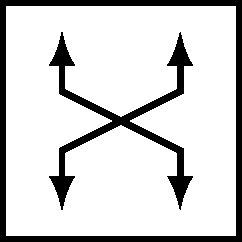
\includegraphics[width=0.9cm]{../common/fig-switch.pdf}
}
\providecommand{\router}{%
    
\includegraphics[width=0.9cm]{../common/fig-router.pdf}
}

% FIXME: scenario where 10.0.2.9 is machine A, then machine B
% FIXME: scenario where machine A and B both think they are 10.0.2.9
\begin{frame}[fragile]{}
\begin{tikzpicture}
\tikzset{
    computer/.style={inner sep=0mm,outer sep=0mm,execute at begin node={\computer}},
    computer alt/.style={inner sep=0mm,outer sep=0mm,execute at begin node={\computerAlt}},
    switch/.style={inner sep=0mm,outer sep=0mm,execute at begin node={\switch}},
    router/.style={inner sep=-1mm,outer sep=0mm,execute at begin node={\router},circle},
    connect/.style={draw,very thick,Latex-Latex},
    connect big/.style={draw,ultra thick,Latex-Latex},
    addr label/.style={align=left,font=\fontsize{9}{10}\selectfont\tt},
    arp table/.style={
        tight matrix,
        nodes={minimum height=.6cm},
        column 1/.style={nodes={text width=2.05cm,font=\small\tt}},
        column 2/.style={nodes={text width=1.75cm,font=\small\tt}},
        %row 1/.style={nodes={font=\small}},
    },
}
\begin{scope}[name prefix=first-]
    \node[computer,label={[addr label]north:MAC 77:\ldots:BB\\IP 10.0.2.2}] (n1-from) at (0, 0) {};
    \node[computer alt,label={[addr label]south:MAC 99:\ldots:BA\\IP 10.0.2.9}] (n1-to) at (0, -4) {};
    \node[switch] (sw) at (0, -2) {};
    \draw[connect] (n1-from) -- (sw);
    \draw[connect] (n1-to) -- (sw);
    \matrix[arp table,label={[label distance=0mm]north:.2's ARP table},inner sep=0mm,fill=white] 
        (arp table) at (2.75, -0.5) {
        10.0.2.9 \& 99:\ldots:BA \\
    };
\end{scope}
\begin{visibleenv}<2->
\draw[line width=2mm,black!50,dashed] (5.3, 2) -- ++(0, -8);
\begin{scope}[name prefix=second-,xshift=7cm]
    \node[computer,label={[addr label]north:MAC 77:\ldots:BB\\IP 10.0.2.2}] (n1-from) at (0, 0) {};
    \node[computer,label={[addr label]south:MAC \myemph<2>{CC:\ldots:01}\\IP 10.0.2.9}] (n1-to) at (2, -4) {};
    \node[switch] (sw) at (0, -2) {};
    \draw[connect] (n1-from) -- (sw);
    \draw[connect] (n1-to) -- (sw);
    \matrix[arp table,label={[label distance=0mm]north:.2's ARP table},inner sep=0mm,fill=white] 
        (arp table) at (2.75, -0.5) {
        10.0.2.9 \& |[alias=wrong mac box,alt=<2>{fill=red!10}]| 99:\ldots:BA \\
    };
    \begin{visibleenv}<2>
        \node[anchor=north,draw=red,very thick,align=left] at ([yshift=-.1cm]wrong mac box.south) {
            old entry prevents 10.0.2.2 \\
            from contacting new machine
        };
    \end{visibleenv}
\end{scope}
\node[anchor=south] at (2, 2) {Monday};
\node[anchor=south] at (8, 2) {Tuesday};
\end{visibleenv}
\end{tikzpicture}
\end{frame}

\begin{frame}{gratituous ARP requests}
    \begin{itemize}
    \item solution: send \textit{unsolicited} ARP messages
    \vspace{.5cm}
    \item CC:\ldots:01$\rightarrow$FF:\ldots:FF: request: who has 10.0.2.9, tell 10.0.2.9=CC:\ldots:01 
    \vspace{.5cm}
    \item<2-> request not reply b/c concerns about old/broken implementations
        \begin{itemize}
        \item ICMPv6 ND fixes this: \\
            message is `advertisement' ($\sim$ reply), not `solicitation' ($\sim$ request)
        \end{itemize}
    \end{itemize}
\end{frame}

\begin{frame}[fragile]{}
\begin{tikzpicture}
\tikzset{
    computer/.style={inner sep=0mm,outer sep=0mm,execute at begin node={\computer}},
    computer alt/.style={inner sep=0mm,outer sep=0mm,execute at begin node={\computerAlt}},
    switch/.style={inner sep=0mm,outer sep=0mm,execute at begin node={\switch}},
    router/.style={inner sep=-1mm,outer sep=0mm,execute at begin node={\router},circle},
    connect/.style={draw,very thick,Latex-Latex},
    connect big/.style={draw,ultra thick,Latex-Latex},
    addr label/.style={align=left,font=\fontsize{9}{10}\selectfont\tt},
    arp table/.style={
        tight matrix,
        nodes={minimum height=.6cm},
        column 1/.style={nodes={text width=2.05cm,font=\small\tt}},
        column 2/.style={nodes={text width=1.75cm,font=\small\tt}},
        %row 1/.style={nodes={font=\small}},
    },
}
\begin{scope}
    \node[computer,label={[addr label]north:MAC 77:\ldots:BB\\IP 10.0.2.2}] (n1-from) at (0, 0) {};
    \node[computer alt,label={[addr label]south:MAC 99:\ldots:BA\\IP \myemph<2>{10.0.2.9}}] (n1-toA) at (-2, -4) {};
    \node[computer alt,label={[addr label]south:MAC 09:\ldots:FE\\IP \myemph<2>{10.0.2.9}}] (n1-toB) at (2, -4) {};
    \node[switch] (sw) at (0, -2) {};
    \draw[connect] (n1-from) -- (sw);
    \draw[connect] (n1-toA) -- (sw);
    \draw[connect] (n1-toB) -- (sw);
\end{scope}
\end{tikzpicture}
\end{frame}

\begin{frame}{duplicate addresses}
    \begin{itemize}
    \item recommendations in RFC 5227 {\small ``IPv4 Address Conflict Detection''}
    \vspace{.5cm}
    \item probe for IP address before using it
        \begin{itemize}
        \item and probably give up on address if conflict found
        \end{itemize}
    \item make periodic `gratituous' requests of address
    \item on detecting conflict choose between:
        \begin{itemize}
        \item `defend' address with more gratituous requests
        \item give up address
        \end{itemize}
    \end{itemize}
\end{frame}
